\documentclass[12pt]{article}
\usepackage{xeCJK}%preamble part
\usepackage{graphicx}
\usepackage{multirow}
\usepackage{pdfpages}
\usepackage{indentfirst}
\usepackage[a4paper, inner=1.5cm, outer=3cm, top=2cm, bottom=3cm, bindingoffset=1cm]{geometry}
\usepackage{epstopdf}
\usepackage{listings}
\usepackage{array}
\usepackage{color}
\usepackage{fontspec}
\usepackage{caption}
\usepackage{subcaption}
\usepackage{diagbox}
\usepackage{bm}
\usepackage{gensymb}
\usepackage{todonotes}
\usepackage{amsmath, amsthm, amssymb}
\usepackage[citecolor=blue]{hyperref}
\newtheorem{definition}{Definition}
\newtheorem{thm}{Theorem}[section]
\newtheorem{cor}[thm]{Corollary}
\newtheorem{lem}[thm]{Lemma}
\newtheorem{remark}[thm]{remark}
\DeclareMathOperator{\sgn}{sgn}
\theoremstyle{remark}
\newtheorem*{rem}{Remark}
\usepackage{makecell}
\setCJKmainfont[BoldFont={SimHei}]{SimSun}
\setCJKmonofont{SimSun}
\setmainfont{Times New Roman}
\newCJKfontfamily[hei]\heiti{SimHei}
\setlength{\extrarowheight}{4pt}
\setlength{\parindent}{1cm}
\definecolor{codegreen}{rgb}{0,0.6,0}
\definecolor{codegray}{rgb}{0.5,0.5,0.5}
\definecolor{codepurple}{rgb}{0.58,0,0.82}
\definecolor{backcolour}{rgb}{0.95,0.95,0.92}
\lstdefinestyle{mystyle}{
    backgroundcolor=\color{backcolour},
    commentstyle=\color{codegreen},
    keywordstyle=\color{magenta},
    numberstyle=\tiny\color{codegray},
    stringstyle=\color{codepurple},
    basicstyle=\footnotesize,
    breakatwhitespace=false,
    breaklines=true,
    captionpos=b,
    keepspaces=true,
    numbers=left,
    numbersep=5pt,
    showspaces=false,
    showstringspaces=false,
    showtabs=false,
    tabsize=2
}
\lstset{style=mystyle}
\begin{document}
\title{\textbf{\fontsize{15.75pt}{\baselineskip}{椭圆型方程实验}}}
\author{数33 赵丰 \\学号:2013012178}
\maketitle
\large
\section{题目}
\includepdf{practice5.pdf}
\section{解析解}
采用分离变量的方法,假设方程有如下形式的解:
\begin{equation}\label{eq:fx}
u(x,y)=f(x)\sin \pi y.
\end{equation}
代入后得$f(x)$满足如下两点边值问题:
\begin{equation}\label{eq:2b}
\begin{cases}
&-\epsilon f''(x)+\epsilon \pi^2 f(x)+f'(x)=\sin \pi x\\
&f(0)=0,f(1)=0.
\end{cases}
\end{equation}
可以求出相应的齐次ODE方程的两个特解为
\begin{equation}
\lambda_{1,2}=\frac{1\pm \sqrt{1+4\epsilon^2\pi^2}}{2\epsilon}
\end{equation}
从而可以得到式(\ref{eq:2b})的解可以写成:
\begin{equation}
f(x)=d_1 exp(\lambda_1 x)+d_2 exp(\lambda_2 x)+g(x)
\end{equation}
其中g(x)是式(\ref{eq:2b})的一个特解。通过待定
\begin{equation}
g(x)=c_1 \sin \pi x + c_2 \cos \pi x
\end{equation}
可求出$g(x)$进而由边值条件确定$d_1,d_2$,下面的Mathematica代码给出了解析解的表达式:
\begin{lstlisting}[language=Mathematica]
realF[x_] := 
 Module[{c1 = N[2 \[Epsilon]/(1 + 4 \[Epsilon]^2*\[Pi]^2)], 
   c2 = N[-1/(\[Pi] + 4 \[Pi]^3*\[Epsilon]^2)], \[Lambda]1 = 
    N[(1 + Sqrt[
         1 + 4*\[Epsilon]^2*\[Pi]^2])/(2 \[Epsilon])], \[Lambda]2 = 
    N[(1 - Sqrt[1 + 4*\[Epsilon]^2*\[Pi]^2])/(2 \[Epsilon])], 
   specialF, d1, d2}, 
  specialF = 
   c1*Sin[\[Pi] x] + c2*Cos[\[Pi] x]; {d1, d2} = {y1, y2} /. 
    Solve[{y1 + y2 == -c2, 
       y1*Exp[\[Lambda]1] + y2*Exp[\[Lambda]2] == c2}, {y1, y2}][[1]];
   d1*Exp[\[Lambda]1*x] + d2*Exp[\[Lambda]2*x] + specialF]
\end{lstlisting}
\section{数值格式}
采用指数型差分格式,设:
\begin{equation}
\sigma=\frac{h}{2\epsilon}\coth{\frac{h}{2\epsilon}}
\end{equation}
则数值格式为:
\begin{equation}
-\epsilon \sigma \frac{(\delta_x^2+\delta_y^2)u_{i,j}}{h^2}+\frac{u_{i+1,j}-u_{i-1,j}}{2h}=\sin(\pi ih)\cos(\pi jh).
\end{equation}
\begin{remark}
注意到$\sigma\to 1,\text{as } h\to 0$,所以指数型差分格式是对五点差分格式的修正。
\end{remark}
利用以上数值格式设计Mathematica程序求解给定的椭圆问题,代码如下所示:
\begin{lstlisting}[language=Mathematica]
(*initialization of parameter*)
\[Epsilon] = 0.01;
N1 = 20;
h = 1/(N1 + 1);
s = SparseArray[{{N1*N1, N1*N1} -> 0}];
b = Table[0, {i, N1*N1}];
(*Exponential Scheme to update s and b*)
\[Sigma] = N[h*Coth[h/(2*\[Epsilon])]/(2*\[Epsilon])];
For[i = 0, i <= N1 - 1, i++,
 For[j = 0, j <= N1 - 1, j++,
  s[[N1*j + i + 1, N1*j + i + 1]] = 4 \[Sigma];
  b[[N1*j + i + 1]] = 
   N[Sin[\[Pi]*(i + 1)/(N1 + 1)]*
     Sin[\[Pi]*(j + 1)/(N1 + 1)]/(\[Epsilon]*(N1 + 1)^2)];
  If[i < N1 - 1,
    s[[N1*j + i + 1, N1*j + i + 2]] = -\[Sigma] + h/(2*\[Epsilon]);]
   If[i > 0,
    s[[N1*j + i + 1, N1*j + i]] = -\[Sigma] - h/(2*\[Epsilon]);]
   If[j < N1 - 1,
    s[[N1*j + i + 1, N1*(j + 1) + i + 1]] = -\[Sigma];]
   If[j > 0,
    s[[N1*j + i + 1, N1*(j - 1) + i + 1]] = -\[Sigma]]
  ]]
(*s is Sparse Matrix, Solver s*x=b *)
result = LinearSolve[s, b];
result2D = 
  Table[result[[(j - 1)*N1 + i + 1]], {j, 1, N1}, {i, 0, N1 - 1}];
\end{lstlisting}
\section{结果分析}
下面取不同的h和$\epsilon$比较指数型差分格式和一般五点差分格式的数值误差,采用各点误差的绝对值的平均数为衡量标准(相当于$\mathbb{L}^2$范数)
\begin{table}[h]
\centering
\begin{tabular}{c|ccc}
\hline
\diagbox{$\epsilon$}{error}{h} &1/21&1/51&1/101\\ \hline
0.1&9.4E-4&1.5E-4&3.8E-5\\
0.01&0.014&0.0013&3.5E-4\\
0.001&0.17&0.036&0.008\\
\hline
\end{tabular}
\caption{五点差分格式解算结果}
\end{table}

由上表可以看出,减小空间步长可以降低误差,通过log-log图可以估计出五点差分格式的数值精度约为$O(h^2)$,与理论结果一致。但随着$\epsilon$的减小,相同步长条件下误差迅速增大。
下面画出$\epsilon=0.001,h=1/101$时数值解与真实解的差别的矩阵图:
\begin{figure}[h]
\centering
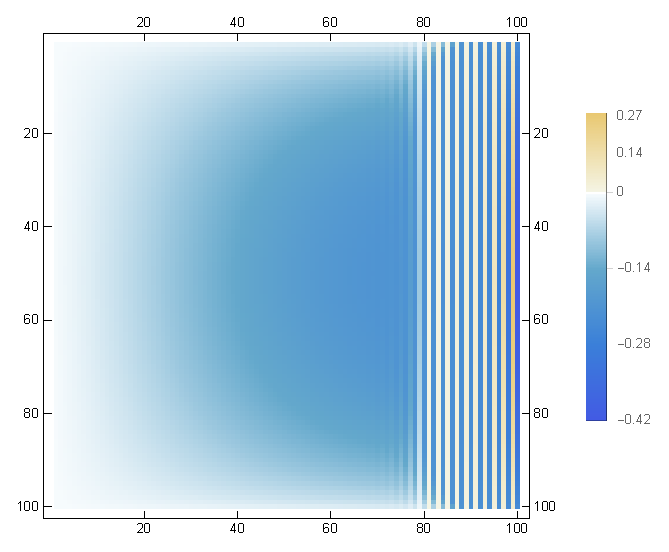
\includegraphics[width=300pt]{5point.eps}
\end{figure}

由上图可以看到,在x接近1的地方,数值解出现了震荡的现象,这说明所求解的问题在x=1处有边界层,通过式(\ref{eq:fx})分析解析解f(x)的在x=1处的性质可知,随着h的减小,f(x)在1附近的导数的绝对值会变大,如下图所示:
\begin{figure}[h]
\centering
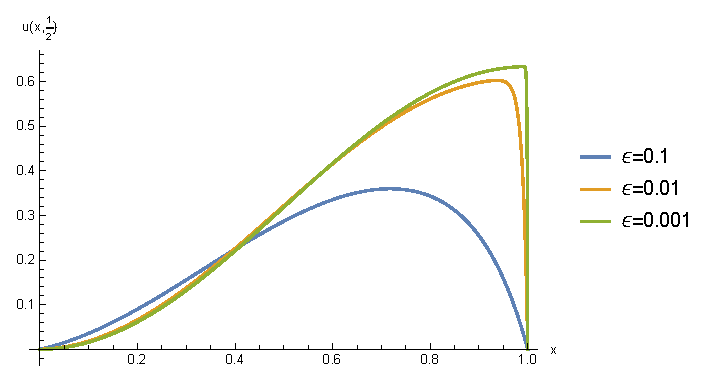
\includegraphics[width=350pt]{boundaryLayer.eps}
\end{figure}
\newpage
下面用指数型差分格式求解该问题:
\begin{table}[h]
\centering
\begin{tabular}{c|ccc}
\hline
\diagbox{$\epsilon$}{error}{h} &1/21&1/51&1/101\\ \hline
0.1&5.6E-4&9.0E-5&2.3E-5\\
0.01&0.007&0.0016&4E-4\\
0.001&0.012&0.005&0.002\\
\hline
\end{tabular}
\caption{指数型差分格式解算结果}
\end{table}


从上表可以看出,对于较小的$\epsilon$,指数型差分格式仍具有较高精度,对$\epsilon=0.001,h=1/101$时数值解与真实解的差别作矩阵图如下:
\begin{figure}[h]
\centering
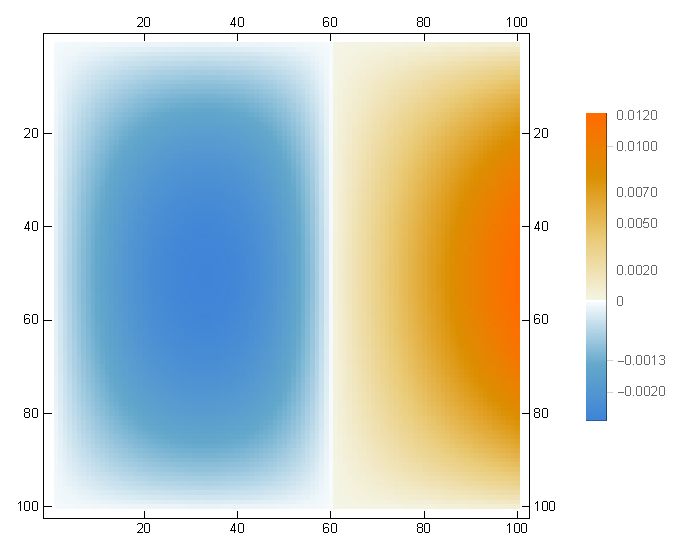
\includegraphics[width=300pt]{Exponentialpoint.eps}
\end{figure}

从上图可看出,使用指数型差分格式消除了x=1附近的振荡现象。
\end{document}
